\chapter{Fundamente teoretice}
\label{cap:fund-teoretice}

În cadrul acestui capitol vor fi prezentate elementele care stau la baza metodei descrise în cadrul acestui proiect. În primele doua secțiuni vor fi definite despărțirea în silabe și tiparele secvențiale, urmând ca în a treia secțiune să fie definit conceptul de tipar secvențial frecvent la nivelul cuvintelor. În cadrul ultimei secțiuni va fi descris BIDE, un algoritm care identifică tipare secvențiale frecvente.

\section{Despărțirea în silabe (silabisirea)}

Prin silabisire se înțelege a procesul de a despărți în silabe un cuvânt. Înainte de a oferi câteva exemple, este necesară o clarificare a conceptului de silabă. 

\begin{defi}
\textbf{Silaba} se definește ca fiind un segment din lanțul vorbirii compus din unul sau mai multe foneme (sunete elementare) pronunțate neîntrerupt într-un singur efort respirator. Orice silabă are ca element principal inevitabil o vocală sau, în unele limbi, o consoană sonantă). Elementul principal poate fi însoțit de consoane, semivocale sau grupuri consonantice și semivocalice dispuse înainte, după, sau de ambele părți ale acestuia. \footnote{http://ro.wikipedia.org/wiki/Silabă}
\end{defi} 

Deasemenea, trebuie menționat că silabisirea nu poate fi definită pe baza unui set rigid de reguli, chiar dacă în majoritatea cazurilor există un asemenea set de reguli. Această ambiguitate la nivelul definirii procesului vine din două cauze: 
\begin{enumerate}
\item limbile nu sunt construite artificial, iar ambiguitatea este un atribut intrinsec al lor. 
\item silabisirea este realizată după seturi diferite de reguli, în functie de scopul pentru care este realizată (fonetic sau ortografic).  
\end{enumerate}

Silabisirea fonetică ilustrează cel mai bine definiția de mai sus, dar când vine vorba de silabisirea ortografică trebuie mentionat ca principala utilitate a acestui tip de despărțire în silabe este de natură  estetică.

\begin{ex}
Din punct de vedere fonetic, despărțirea în silabe a cuvântul \textit{inegal} este \textbf{i-ne-gal}, dar din punct de vedere ortografic, utilizând reguli morfologice rezultă despărțirea \textbf{in-e-gal}. 
\end{ex}

\section{Tipare secventiale frecvente}

Tiparele secventiale frecvente sunt acele tipare care se regasesc în cadrul unei colecții de secvențe ordonate de numar minim de ori. Acest numar va fi referit ulterior și ca \textit{suport minim}. 

În cele ce urmează, se va realiza o introducere formală pentru tiparele secvențiale frecvente, urmând ca după această scurtă întroducere să fie ilustrat modul în care o colecție de cuvinte despărțite în silabe poate fi asociată cu o colecție de secvențe.

\begin{defi}
Fie $I = \{i_1, i_2, ...,i_n\}$ alfabetul (un set distinct de elemente) colecției de secvențe. O \textbf{secvență $s$} este definită ca fiind o listă ordonată de elemente din alfabetul $I$:
\begin{equation}
<i_{k_1},i_{k_2}, ...,i_{k_m}>,\ unde \ \forall k_j, 0 \leq j \leq m, k_j \in I.
\end{equation}
\end{defi}

\begin{ex} 
Având alfabetul $I=\{a,b,c,d\}$, o posibilă secvență este $<b,b,a>$.
\end{ex}

\begin{defi} 
Printr-o \textbf{colecție de secvențe $S_{db}$} se înțelege un set de tuple de forma $(id, s)$, unde $id$ este un identificator unic iar $s$ este o secvență. 
\end{defi}

\begin{ex}
Un exemplu de astfel colecție de secvențe este prezentat în cadrul tabelului \ref{table:sdb}
\end{ex}

\begin{table}[h]
\centering    
\begin{tabular}{|c|c|}    
\hline      
$id$ & $s$ \\
\hline                    
1 & $<C,A,A,B,C>$ \\
2 & $<A,B,C,B>$ \\
3 & $<C,A,B,C>$ \\
4 & $<A,B,B,C,A>$ \\
\hline                              
\end{tabular}
\caption{Exemplu de colecție de secvențe}
\label{table:sdb}               
\end{table}

\begin{defi}
Despre o secvență $s_1=<t_1, t_2, ...,t_n>$ se poate spune ca este \textbf{conținută} de o secvență $s_2=<l_1, l_2, ...,l_m>$ dacă $n \leq m$ și $ \exists i,j$ astfel încât $t_1 = l_i, t_n = l_j$ și $\forall k, i \leq k \leq j \implies t_{k-i} = l_k$. Pentru această incluziune a secvențelor se va utiliza ulterior notația $s_1 \subseteq s_2$.
\end{defi}
      
\begin{defi}

Fie $S_{db}$ o colecție de secvențe, iar $T$ multimea tuplelor $(id, s)$ din $S_{db}$, pentru care $s' \subseteq s$. \textbf{Suportul} secvenței $s'$ în cadrul acestei colecții de secvențe este $\vert T \vert$.  Informal, suportul unei secvențe într-o colecție de secvențe este egal cu numarul de secvențe din acea colecție, care conțin secvența respectivă. Pentru suportul secvenței $s$ în cadrul $S_{db}$ se va utiliza notația $sup_{S_{db}}(s)$.
\end{defi}

\begin{defi}
Pornind de la definiția unei secvențe și a suportului acesteia, se poate introduce conceptul de \textbf{tipar secvențial frecvent}. Un tipar secvențial frecvent nu este altceva decât o secvență care în cadrul unei colecții de secvențe $S_{db}$ are un suport mai mare sau egal cu un prag minim. Acest prag minin se mai numește și suport minim.
\end{defi}
\section{De la silabisire la tipare secvețiale frecvente}
Identificare tiparelor descrise anterior prezintă un interes deosebit, cu aplicabilitate într-o multitudine de domenii, iar după cum va fi ilustrat în capitolele urmatoare, tiparele extrase din cuvinte deja despărțite în silabe pot fi utilizate pentru a construi strategii de predicție a silabisirii cuvintelor. 

\begin{ex}
Într-un astfel de scenariu în care se dorește identificarea tiparelor frecvente din cuvinte despărțite în silabe, alfabetul colecției de secvențe este reprezentat de mulțimea tuturor posibilelor silabelor, iar fiecare cuvânt reprezintă o secvență. În cadrul tabelului \ref{table:sdb_words} este prezentată o astfel de colecție de secvențe.
\end{ex}

\begin{table}[h]
\centering    
\begin{tabular}{|c|c|}    
\hline      
$id$ & $s$ \\
\hline
1 & \textit{<li, be, lu, lă>} \\
2 & \textit{<e, li, be, ra, tor>} \\
3 & \textit{<a, ma, tor>}\\
4 & \textit{<ar, ti, col>} \\
5 & \textit{<pro, gra, ma, tor>} \\
6 & \textit{<a, ni, ver, sa, re>} \\
7 & \textit{<vi, sa, re>} \\
8 & \textit{<gra, ma, ti, că>} \\
9 & \textit{<e, va, da, re>} \\
10 & \textit{<ma, re, e>} \\
11 & \textit{<pro, gra, ma, re>} \\
12 & \textit{<gân, di, tor>} \\
13 & \textit{<e, li, tă>} \\
14 & \textit{<sa, re>} \\
15 & \textit{<e, li, cop, ter>} \\
\hline                              
\end{tabular}
\caption{Exemplu de colecție de secvențe construite pe baza unui set de cuvinte despărțite în silabe}
\label{table:sdb_words}               
\end{table}

Pentru colecția de secvențe frecvente din cadrul tabelului \ref{table:sdb_words}, în cadrul tabelului \ref{table:sdb_patterns} sunt ilustrate tiparele frecvente în funcție de diferite valori ale suportului minim. Se va nota cu $(s,sup)$ un tipar frecvent, unde $s$ este tiparul propriu-zis iar $sup$ reprezintă valoarea suportului aceste secvente.

Tiparele identificate dintr-un set mare de cuvinte deja silabisite, pe lângă valoarea lor în contextul analizelor de fonetica și morfologie a limbi, pot fi folosite pentru a automatiza procesul de silabisire, asa cum va fi ilustrat în cadrul capitolului următor.

\begin{table}[h!]
\centering    
\begin{tabular}{|c|l|}    
\hline      
Suport minim & Tipar frecvent\\
\hline
2& $(<a>, 2)$  \\
 & $(<li, be>, 2)$  \\
 & $(<pro, gra, ma>, 2)$  \\
 & $(<ma, re>, 2)$  \\
 & $(<ma, tor>, 2)$  \\
 & $(<ti>, 2)$  \\
 & $(<e, li>, 3)$  \\
 & $(<gra, ma>, 3)$  \\
 & $(<sa, re>, 3)$  \\
 & $(<tor>,4)$  \\
 & $(<li>, 4)$  \\
 & $(<e>, 5)$  \\
 & $(<ma>,5)$  \\
 & $(<re>, 6)$  \\
\hline
3& $(<e, li>, 3)$  \\
 & $(<gra, ma>, 3)$  \\
 & $(<sa, re>, 3)$  \\
 & $(<tor>,4)$  \\
 & $(<li>, 4)$  \\
 & $(<e>, 5)$  \\
 & $(<ma>,5)$  \\
 & $(<re>, 6)$  \\
\hline
4& $(<tor>,4)$  \\
 & $(<li>, 4)$  \\
 & $(<e>, 5)$  \\
 & $(<ma>,5)$  \\
 & $(<re>, 6)$  \\
\hline
5& $(<e>, 5)$  \\
 & $(<ma>,5)$  \\
 & $(<re>, 6)$  \\
\hline
 & $(<re>, 6)$  \\
\hline                              
\end{tabular}
\caption{Exemplu de colecție de secvențe construite pe baza unui set de cuvinte despărțite în silabe}
\label{table:sdb_patterns}               
\end{table}

În cadrul sectiunii următoare se va face o scurtă prezentare a unuia dintre algoritmii performanți, cu ajutorul caruia se pot identifica tipare frecvente. 

\section{Algoritmul BIDE}
Algoritmul BIDE, prezentat în detaliu în \cite{bib:wang2004bide}, este o soluție capabilă să extragă tipare secventiale frecvente inchise.

\begin{defi}
Prin \textbf{tipar secvential închis} se întelege un tipar dintr-un set de tipare pentru care nu exista alt tipar care să-l conțină și să aiba același suport. Formal, $s$ este închis dacă $\forall s' \epsilon S_{db}, \nexists (s \subseteq s' \wedge sup_{S_{db}}(s)=sup_{S_{db}}(s'))$.
\end{defi}  

\begin{defi}
Prin proiecția unei sevențe $s$ într-o colecție de secvente $S_{db}$ se întelege multimea tuturor acelor subsecvente cu care $s$ \textit{se continuă} secvența $s$. De exemplu, în cadrul colecției de secvențe din cadrul \ref{table:sdb}, proiectia secventei $<A,B>$ este {$<C>,<C, B>,<C>,<B, C, A>$}. Pseudo-proiecția secvenței $s$ reprezintă setul indexi ai extensiilor. 
\end{defi}  


\begin{algorithm}[H]
\SetAlgoLined
\SetKwFunction{fse}{frequentSequenceEnumeration}
\SetKwFunction{fs}{frequentSequences}
\fse($S_{db}, sup_{min}, FS$) \\
\KwData{$S_{db}$ o colecție de secvențe, pragul minim de suport $sup_{min}$}
\KwResult{setul complet de tipare secvențiale frecvente FS} 
$FS = \emptyset$ \\
call \fs($S_{db}, \emptyset, sup_{min}, FS$) \\
\KwRet $FS$ \\

\BlankLine
\BlankLine

\SetKwFunction{fs}{frequentSequences}
\fs($s_pS_{db}, s_p, sup_{min}, FS$) \\
\KwData{$s_pS_{db}$ o pseudo proiectie a secvenței $s_p$ în colecția de secvențe $S_{db}$, pragul minim de suport $sup_{min}$}
\KwResult{setul de tipare secvențiale frecvente FS} 

\If{$s_p \neq \emptyset$}{
	$FS = FS \cup S_p$
}

$LF\_s_p =$ elementele frecvente cu care poate fi extinsă $s_p$

\If{$LF\_s_p = \emptyset$} {
\KwRet
}

\For{ $i$ in $LF\_s_p$}{
	$s_p^i = <s_p, i>$ \\
	$s_p^iS_{db}$ = pseudo proiecția secvenței $s_p^i$ în cadrul $s_pS_{db}$ \\
	call \fs($s_p^iS_{db}, s_p^i, sup_{min}, FS$)
}
\caption{Descoperirea tiparelor secvențiale frecvente}
\label{algo:fse}
\end{algorithm}

În cadrul algoritmului \ref{algo:fse} este prezentată idea din spatele algoritmului BIDE. Pe scurt, acesta porneste de la un set de tipare de lungime mică, pe care încearcă recursiv să le \textit{crească} atât timp cat suportul lor rămâne peste pragul minim. Varianta prezentată este mult simplificată, algoritmul BIDE complet identifica doar secvențe frecvente închise și adaugă o serie de tehnici de optimizare, cum ar fi eliminarea rapida a tiparelor care nu mai pot fi \textit{crescute}, eficiență la nivelul utilizarii de memorie dar și performanțe bune ca timp de execuție.

\begin{ex}
Pentru tabelul \ref{table:sdb}, la o trasare a algoritmului \ref{algo:fse} identificarea tiparelor frecvente este ilustrată de figura \ref{fig:bide-algo} (exemplu preluat din \cite{bib:wang2004bide}). În prima fază sunt identificate elementele de lungime 1 ($<A>,<B>,<C>$) si le este calculat suportul. Presupunând că suportul minim este 2, pentru fiecare dintre aceste tipare de lungime 1, se caută extensii în colecția de secvențe. În figura la nivelul 2 sunt prezentate aceste tipare iar alaturi, suportul asociat. Algoritmul avanseaza recursiv pentru fiecare tipar astfel identificat. Nodurile marcate cu linie continuă reprezintă tiparele frecvente închise. 
\end{ex}

\begin{figure}[h]
    \centering
    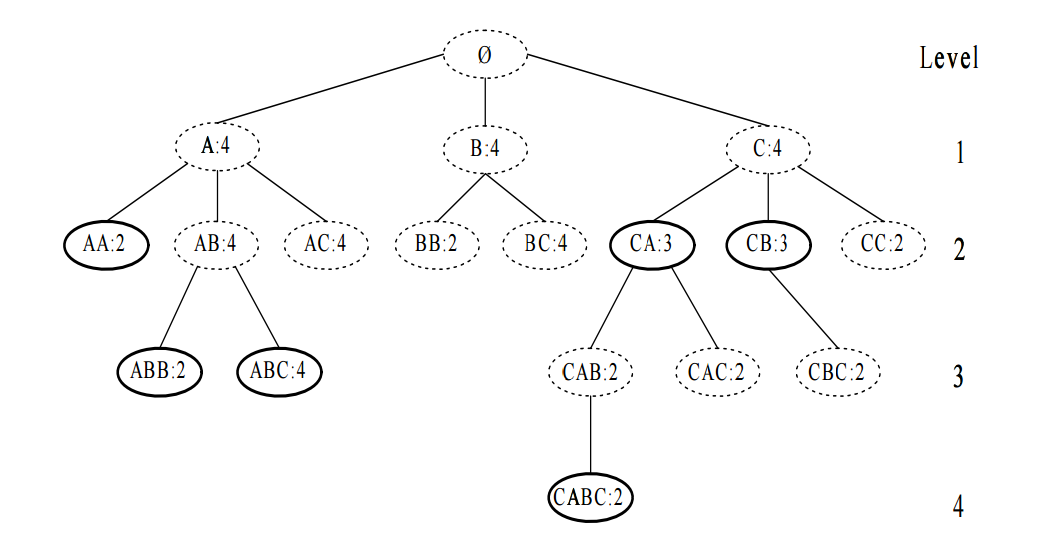
\includegraphics[width=\textwidth]{figures/bide-tree.png}
    \caption{Arborele de constructie a tiparelor frecvente}
    \label{fig:bide-algo}
\end{figure}
